\documentclass{beamer}
\usetheme{default}
\usepackage[utf8]{inputenc}
\usepackage[spanish]{babel}
\usepackage{hyperref}
\usepackage{wrapfig}
\usetheme{Madrid}
\usecolortheme{seahorse}
\usefonttheme{professionalfonts}
\title{The Computer Scientist as Toolsmith II}
\subtitle{by Fred Brooks}
\author{Antonio, Campos, Chavez, Herrero}
\institute{Ingeniería de Software II}
\date{\today}
\begin{document}

\begin{frame}
\titlepage
\end{frame}

\section{Introduccion}
\begin{frame}{Sobre Fred Brooks}

\begin{itemize}
\item Ingeniero de software y científico de la computación 
\item Ph. D en matemática
\item Fundó el departamento de Computer Science en la Universidad de Carolina del Norte
\item Dirigió el desarrollo del sistema operativo OS/360 de IBM
\item The Mythical Man-Month
\item No Silver Bullet
\item Brooks' law: ``Adding manpower to a late software project makes it later.''
\end{itemize}
\end{frame}

\begin{frame}{Premios}
\begin{itemize}
\item National Medal of Technology - 1985
\item ACM Allen Newell Award - 1994
\item Turing Award - 1999
\end{itemize}
\begin{center}
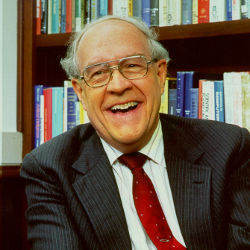
\includegraphics[height=.50\textheight]{Brooks.jpg}
\end{center}
\end{frame}

\begin{frame}{¿Ciencia?}
\begin{quote}
La ciencia es una rama del estudio que se ocupa de la observación y
clasificación de \textbf{hechos}, especialmente del establecimiento y
formulación cuantitativa de \textbf{leyes} generales verificables.
\textnormal{(Diccionario Webster)}
\end{quote}
\begin{itemize}
\item Los \textbf{científicos} construyen para estudiar, los
	\textbf{ingenieros} estudian para construir.
\end{itemize}
\end{frame}

\begin{frame}{\emph{Computer Science}}
\begin{itemize}
\item Se dice que "todo lo que se llama a sí mismo ciencia, no es una ciencia"
\item \emph{Computer Science} no es una disciplina científica; es una
	\textbf{ingeniería relacionada con crear cosas abstractas}
\end{itemize}
\end{frame}

\begin{frame}{¿Qué somos?}
\begin{block}{}
	\begin{center}
	\LARGE Somos \textbf{toolsmiths}: Personas que hacen herramientas.
	\end{center}
\end{block}
\begin{itemize}
\item Somos exitosos si los usuarios de nuestras herramientas son exitosos.
\end{itemize}
\end{frame}


\begin{frame}{Cómo puede un nombre despistarnos?}
\begin{center}
\begin{enumerate}
\item Tendemos a pensar que una ciencia tiene mayor 'valor'
que una ingeniería...
\item Un nuevo hecho, una nueva ley es un logro que
merece publicación.
Si reconocemos nuestros artefactos como herramientas, 
probamos su uso y costo, no por su novedad.
\item Tendemos a olvidar a nuestros usuarios y sus problemas reales,
abstraemos demasiado dejando detrás la esencia del problema real.
\end{enumerate}
\end{center}
\end{frame}

\begin{frame}{La parte Computer está bien}
\begin{itemize}
\item[] La diferencia clave entre ciencas de la computación
y el resto de las ciencias es que somos especialistas en problemas 
que se caracterizan por ser de complejidad arbitraria.
\item[] Matemáticos se escandalizan por la complejidad. 
\item[] Mientras físicos o biólogos se escandalizan por 
la arbitrariedad.
\end{itemize}
\end{frame}

\begin{frame}{Evolución de la Inteligencia Artificial}
\begin{itemize}
\item "Haremos máquinas que piensan; haremos Mentes Gigantes"
\item Se ha logrado sorprendentemente poco por el tiempo y la inversión realizada.
\item Estos años de experiencia dieron a los trabajadores en AI 
un respeto profundo por el poder de la mente humana.
\item Es momento de reconocer que los objetivos originales de AI 
no fueron extremadamente difíciles,
fueron objetivos que, aunque glamorosos y motivantes, 
enviaron a la disciplina en una dirección equivocada.
\item En vez de intentar reemplazar la mente humana con máquinas, 
deberíamos estudiar cómo amplificar la mente humana usandolas.
\item Intelligence Amplifying $>$ Artificial Intelligence
\end{itemize}
\end{frame}

\begin{frame}{Colaboración}
\begin{itemize}
\item Debemos asociarnos con aquellos que usarán esas herramientas, aquellos cuya ``inteligencia'' queremos aumentar.
\item Trabajando en los problemas de otras disciplinas, con el fin de colaborar puede, de muchas formas, ayudarnos como computadores científicos.
	\begin{itemize}
	\item Lidiamos con problemas relevantes, y no con ``problemas/ejercicios de juguete''
	\item No nos engañamos con nuestros éxitos o fracasos
	\item Enfrentamos el problema en su totalidad
	\item Y esto nos fuerza a desarrollar áreas que nunca hubieramos investigado
	\item Es divertido (?)
	\end{itemize}
\item En todo trabajo interdisciplinario tiene un costo la ``interacción'': un cuarto del tiempo se va en trabajo inevitable ``de rutina"
\item Se necesita que los expertos de cada disciplina aprendan sobre la otra
\item El proceso de colaboración al crear una herramienta útil debe ser un proceso iterativo para lograr ser exitoso

\end{itemize}
\end{frame}

\begin{frame}{Preguntas interesantes interesantes}
\begin{itemize}
\item Como sociedad, a qué le damos importancia ?
\item Sysadmin de la NASA: ``I'm not worried about the space program. I'm worried about America. Our nation has become a nation of consumption. Entretainment and recreation are the most importan things for the future. God help us!''
\item La televisión es inherentemente no-social, y conocemos el valor de interactuar con las personas
\item Los greigos se preguntaban sobre cada aspecto de la vida: Es verdad ? Es bello ? Es bueno ?
\item Antes de la television, la gente iba de visita, inventaba cosas, creaba musica, juegos, leia, hacia deporte, observaba la naturaleza

\end{itemize}
\end{frame}

\begin{frame}{¿Qué podemos hacer ?}
\begin{itemize}
\item La creación humana puede ser: hermoso u horrible, maravillosamente bueno o horriblemente maligno
\item Como dijo Jesús, depende del corazón de cada uno
\item Como el apostol Pablo dijo, debemos hacer algo que sea:

	\begin{itemize}
	\item Noble
	\item Justo
	\item Puro
	\item Apasionante
	\item Honorable

	\end{itemize}

\end{itemize}
\end{frame}


\end{document}
